\documentclass[10pt]{article}
\usepackage[margin=1.2in]{geometry}
\usepackage{graphicx}
\graphicspath{{./Figures/}}
\usepackage{tikz}
\usetikzlibrary{arrows}
\tikzset{>=latex}
\usepackage{amsmath,amsfonts,amssymb}
\usepackage[hidelinks,colorlinks,linkcolor={blue!50!black},urlcolor={blue!80!black}]{hyperref}
\renewcommand{\baselinestretch}{1.4}
\setlength\parindent{0pt}
\everymath{\displaystyle}
\author{
  Brian Chu\\
  \texttt{github.com/}
  \and
  Brian Faure\\
  \texttt{github.com/bfaure}
  \and
  Nathan Kjer\\
  \texttt{github.com/nathankjer}
  \and
  Adam Massoud\\
  \texttt{github.com/amassoud20}
  \and
  Viswanatha Subramanian\\
  \texttt{github.com/}
  \and
  Wanshu Sun\\
  \texttt{github.com/waynesun95}
  \and
  Luke Wielgus\\
  \texttt{github.com/lukewielgus}
}
\date{}
\title{\centerline{\includegraphics[scale=2]{Wikipedia-logo-v2.pdf}}\vspace{3em}WikiClassify}
\begin{document}
\clearpage\maketitle
\thispagestyle{empty}
\newpage
\setcounter{page}{1}
\tableofcontents
\section{Definitions}
\centerline{\includegraphics[scale=0.5]{markup.png}}
\subsection*{Wiki Markup}
\href{https://en.wikipedia.org/wiki/Help:Wiki_markup}{Wiki Markup} is a simple markup language. It is the format in which all Wikipedia pages are stored. While being very similar in syntax, Wiki Markup serves as a simpler, templated interface to HTML.
\section{Project Description}
\subsection{Problem Domain}
\hspace*{28pt}Wikipedia is a crowdsourced online encyclopedia founded in 2001. With the goal of centralizing all of human knowledge, it attempts to be a neutral, global, and uncensored source of free information. As of 2016, Wikipedia is ranked number seven on the world’s most popular websites, holds a top priority on search engines, and has been estimated to be worth hundreds of billions of dollars. Furthermore, articles on Wikipedia have been cited in hundreds of court cases. Reliable or not, Wikipedia is heavily used as a result of its high quality content across a broad range of subjects.\\
\hspace*{28pt}Anyone can edit Wikipedia, which is the primary reason why it is one of the largest online encyclopedias in the world. However, this has numerous trade-offs. Destructive editing is a common problem that can go unnoticed for extended periods of time. In addition, articles are frequently cited with unreliable sources, or not cited at all. Furthermore, Wikipedia has editor bias; 90\% of Wikipedians are male, 40\% of the world's population has access to the internet (Wikipedia can only be edited from a selection of 40\% of the world's population), editors are often from white collar backgrounds, have stronger technical abilities, are more frequently from the Northern Hemisphere, and common languages and Western culture are more heavily represented. With such an editor bias, there is a larger probability of the content being misrepresented or not being of acceptable quality.\\
\hspace*{28pt}Thus, despite being one of the most popular and heavily accessed online encyclopedias, the biggest issue with Wikipedia is that not all of its content may be of satisfactory quality.
\subsection{Specific Problems}
\hspace*{28pt}Wikipedia's quality is not consistent. It is too large for a human to proofread and too hard for a computer to edit. Therefore, a text classifier is desired so that content needing the most attention can be found. If there was to be some sort of software or system in place that could rate Wikipedia's quality autonomously, a user could easily determine which Wikipedia articles have satisfactory quality for viewing. Thus, if this solution was successfully implemented, any user who would like to access Wikipedia can get high quality content. Furthermore, besides typical everyday Wikipedia viewers, Wikipedia itself could benefit from such a system, as they would have an easy solution to determining whether or not articles are of acceptable quality.
\subsection{Problem Summary}
\begin{itemize}
\item Input text and receive output parameters that classify the text based on our machine learning algorithm.
\item Uncover biases hidden in Wikipedia rating schema.
\item Compare accuracy of multiple input text articles.
\item Check text for historical accuracy/bias.
\item Compare different portions of Wikipedia based on article quality.
\end{itemize}
\section{Plan of work}
\centerline{\fbox{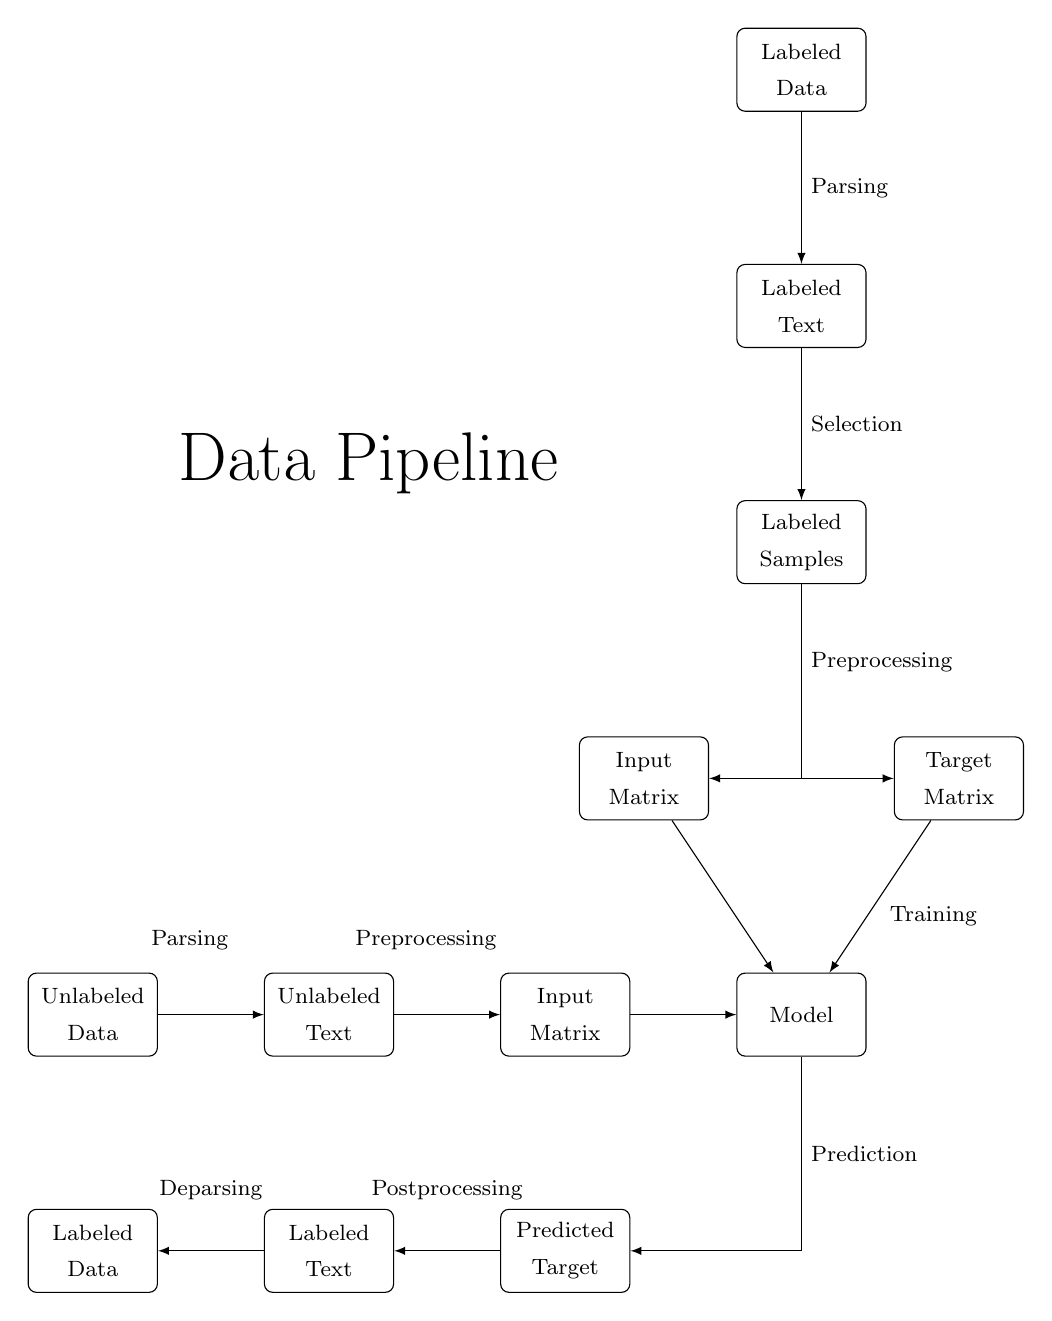
\begin{tikzpicture}[->,auto,align=center]
\tikzstyle{obj} = [font=\footnotesize,rectangle,draw,align=center, text width=4em, minimum height = 3em,rounded corners=3pt]
\node at (-5.5, 7) {\Huge Data Pipeline};
\node[obj] (raw) at (0,12) {Labeled Data};
\node[obj] (pars) at (0,9) {Labeled Text};
\node[obj] (sel) at (0,6) {Labeled Samples};
\node[obj] (in) at (-2,3) {Input Matrix};
\node[obj] (targ) at (2,3) {Target Matrix};
\node[obj] (mod) at (0,0) {Model};
\node[obj] (uraw) at (-9,0) {Unlabeled Data};
\node[obj] (upars) at (-6,0) {Unlabeled Text};\\
\node[obj] (uin) at (-3,0) {Input Matrix};
\node[obj] (utarg) at (-3,-3) {Predicted Target};
\node[obj] (ulpars) at (-6,-3) {Labeled Text};
\node[obj] (ulraw) at (-9,-3) {Labeled Data};
\draw (raw) -> (pars) node[pos=0.5] {\footnotesize Parsing};
\draw (pars) -> (sel) node[pos=0.5] {\footnotesize Selection};
\draw (sel) |- (in);
\draw (sel) |- (targ) node[pos=0.2] {\footnotesize Preprocessing};
\draw (in) -> (mod);
\draw (targ) -> (mod) node[pos=0.5] {\footnotesize Training};
\draw (uraw) -> (upars) node[pos=0.3,above=2em] {\footnotesize Parsing};
\draw (upars) -> (uin) node[pos=0.3,above=2em] {\footnotesize Preprocessing};
\draw (uin) -> (mod);
\draw (mod) |- (utarg) node[pos=0.25] {\footnotesize Prediction};
\draw (utarg) -> (ulpars) node[pos=0.5,above=1.5em] {\footnotesize Postprocessing};
\draw (ulpars) -> (ulraw) node[pos=0.5,above=1.5em] {\footnotesize Deparsing};
\end{tikzpicture}}}
The figure above gives a general outline to the process that we will follow to achieve our solution. The following describes each iteration of the process in further detail.\\[2ex]
\textbf{Raw Data:} The direct Wikipedia data dump. A monthly snapshot of Wikipedia is available from https://dumps.wikimedia.org/, saved as a gzipped tarball of an XML file.\\
\textbf{Target Data:} Classified text sequences that have been parsed from the XML file. The classifications are from articles containing tags such as those listed below.\\
\textbf{Preprocessed Data:} Classified text sequences (strings) are truncated into fixed lengths and converted into a numeric matrix format character­wise and preprocessed.\\
\textbf{Transformed Data:} Dimensions of the preprocessed matrix are reduced\\
\textbf{Patterns:} The machine learning will create a model that best reconstructs the targets from the inputs. This model will be used to predict values where targets do not yet exist. We will know our program has succeeded when the model’s cost, or error is sufficiently low.\\
\textbf{Knowledge:} The backtested results of classifications are visualized and delivered to the user for interpretation.\\
The table below holds the pairs we split into as well as our “general” starting tasks. The way that we wish to work on the project is more so of helping out on each part, with our starting points being the ones listed below.
\end{document}